%! Author = mariuszindel
%! Date = 02.11.20

\section{Attributes}

\subsection{Übersicht}
\begin{itemize}
    \item Erweitern bestehende Attribute wie z.B. «public», «static», «abstract» oder «sealed»
    \item Basisklasse «System.Attribute»
    \item Anwendungsfälle
    \begin{itemize}
        \item Object-relational Mapping
        \item Serialisierung (WCF, XML, etc.)
        \item Security und Zugriffsteuerung
        \item Dokumentation, etc.
    \end{itemize}
    \item Arten von Attributen
    \begin{itemize}
        \item «Intrinsic» Attribute
        \item «Custom» Attribute
    \end{itemize}
\end{itemize}
\begin{lstlisting}
[DataContract, Serializable] [Obsolete] // Etc.
public class Auto {
    [DataMember]
    public string Marke { get; set; }

    [DataMember]
    public string Typ { get; set; }}
\end{lstlisting}

\subsubsection{Syntax}
\begin{itemize}
    \item Beliebig viele Attribute möglich
    \begin{itemize}
        \item $[DataContract][Serializable] $oder$ [DataContract, Serializable]$
    \end{itemize}
    \item Je nach Implementation eines Attributes kann es mehrfach angewandt werden
    \item Parameter / Werte müssen vom Compiler berechenbar sein
    \begin{itemize}
        \item Ohne $\rightarrow$ [DataContract]
        \item Named Parameters $\rightarrow$ [DataContract(Name = "AutoClass")]
        \item Positional Parameters $\rightarrow$ [Obsolete("Alt!", true)]
        \item Mixed $\rightarrow$ [Obsolete("Alt!", IsError = true)]
    \end{itemize}
\end{itemize}

\subsubsection{Reflection}
\begin{itemize}
    \item Attribute können über Reflection abgefragt werden
    \item Definiert durch Interface «ICustomAttributeProvider»
    \begin{itemize}
        \item IsDefined-Methode prüft ob Attribut vorhanden
        \item GetCustomAttributes-Methode liefert Liste aller Attribute
    \end{itemize}
    \item Implementierende Klassen
    \begin{itemize}
        \item Assembly / Module
        \item Type
        \item MemberInfo
        \item ParameterInfo
    \end{itemize}
\end{itemize}


\subsection{Beispiel Custom Attribute}
\subsubsection{Deklaration}
\begin{center}
    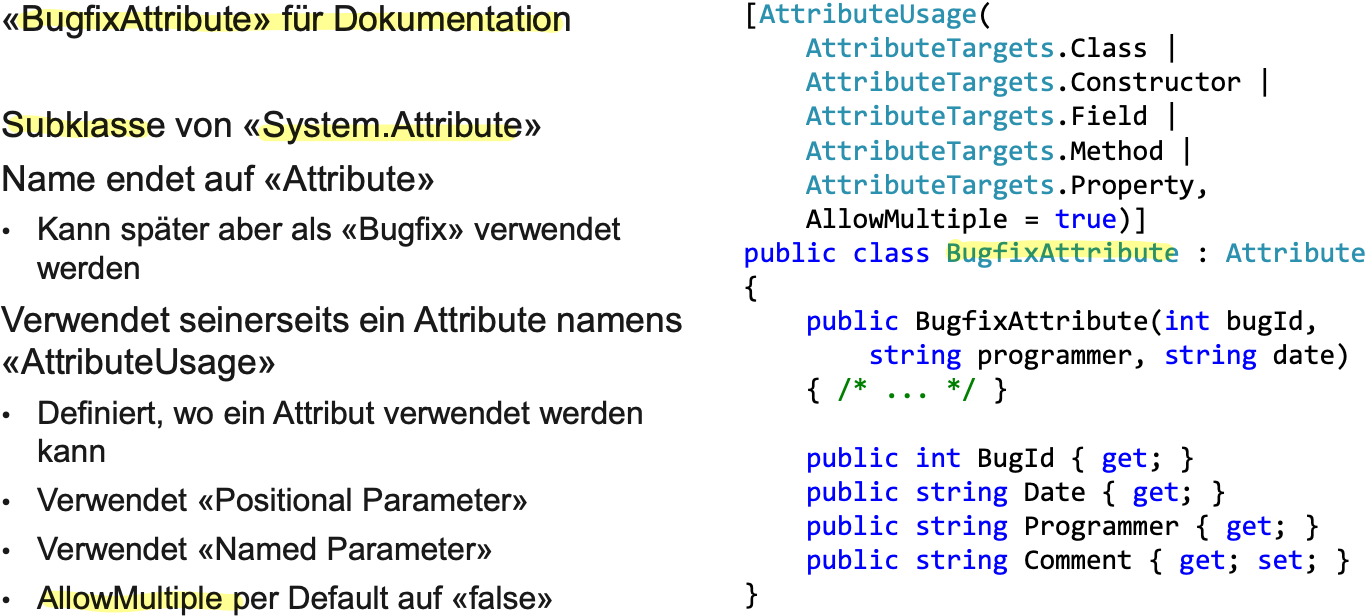
\includegraphics[scale=.35]{graphic/ref attr/deklaration.png}
\end{center}
\vspace{-8pt}

\subsubsection{Anwendung}
\begin{center}
    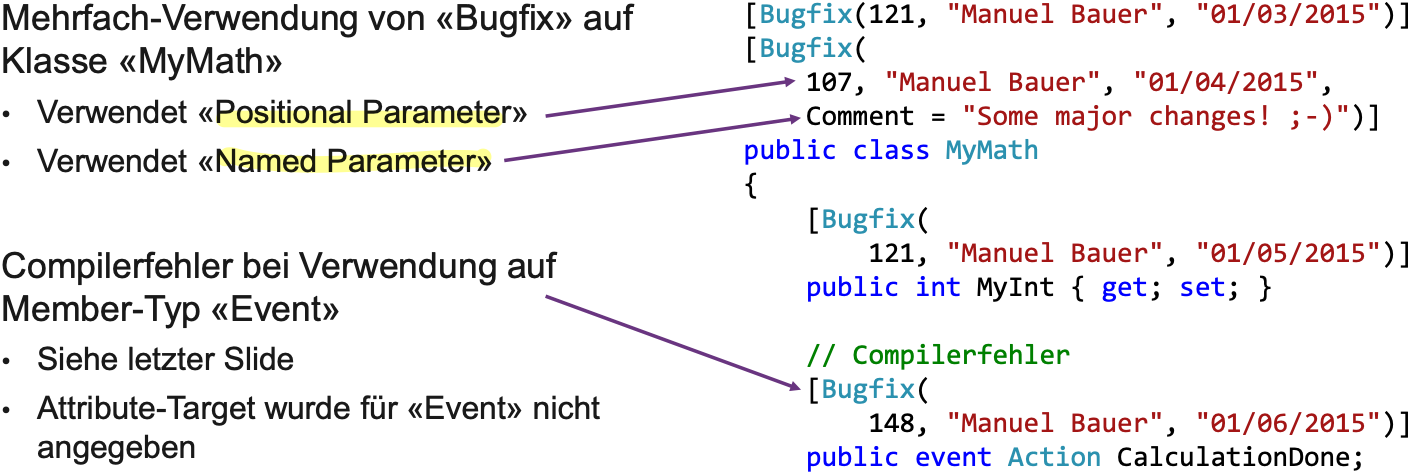
\includegraphics[scale=.35]{graphic/ref attr/anwendung.png}
\end{center}
\vspace{-8pt}

\subsubsection{Abfrage via Reflection}
\begin{center}
    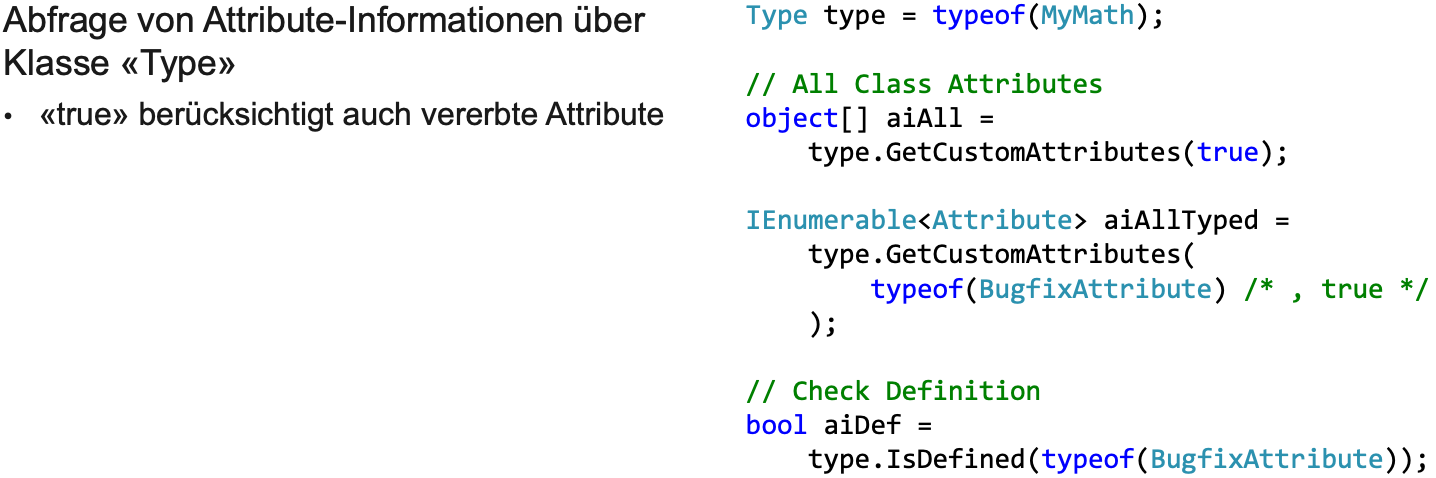
\includegraphics[scale=.35]{graphic/ref attr/abfrage.png}
\end{center}
\vspace{-8pt}


